\section{Sicherheit}
\label{sec:sicherheit_basics}

Wie aus der Abbildung in Abschnitt \ref{subsec:overlay_netzwerke} \textit{\nameref{subsec:overlay_netzwerke}} ersichtlich ist, ist das Overlay-Netzwerk die oberste Schicht des Peer-to-Peer-Netzwerks. Es sorgt dafür, dass sich die Teilnehmer des Netzwerks finden können. Die eigentliche Kommunikation, also das Senden und Empfangen von Nachrichten, erfolgt jedoch über das Internet. Da das Internet ein öffentliches Netzwerk ist, besteht die Gefahr, dass die Nachrichten abgefangen und mitgelesen werden können. Die Nachrichten müssen über Verteilerknoten oder Access Points übertragen werden, die nicht vertrauenswürdig sind. Um ein Mitlesen oder Verändern der Nachrichten zu verhindern, muss die Kommunikation abgesichert werden. 

Mittels Kryptografie kann die Vertraulichkeit, Integrität und Authentizität der Kommunikation gewährleistet werden \Parencite[S. 7]{Hellmann_IT-Sicherheit}.


\subsection{Vertraulichkeit}
\label{subsec:vertraulichkeit_basics}

Die Vertraulichkeit der Kommunikation wird durch Verschlüsselung gewährleistet. Man unterschiedet zwei Formen der Kryptografie: \textit{symmetrische} und \textit{asymmetrische} Kryptografie. Bei der \textit{symmetrischen} Kryptografie wird ein und derselbe Schlüssel zum Verschlüsseln und Entschlüsseln der Nachricht verwendet. Der Sender der Nachricht verschlüsselt die Nachricht mit einem Schlüssel und sendet die nun verschlüsselte Nachricht an den Empfänger. Der Empfänger kann die Nachricht mit dem gleichen Schlüssel entschlüsseln. Dadurch kann ein Angreifer, der die Nachricht abfängt, diese nicht entschlüsseln, da er den Schlüssel nicht kennt. Abbildung \ref{fig:symmetrische_verschluesselung} zeigt den Ablauf der symmetrischen Verschlüsselung.

\begin{center}
    \captionsetup{type=figure}
    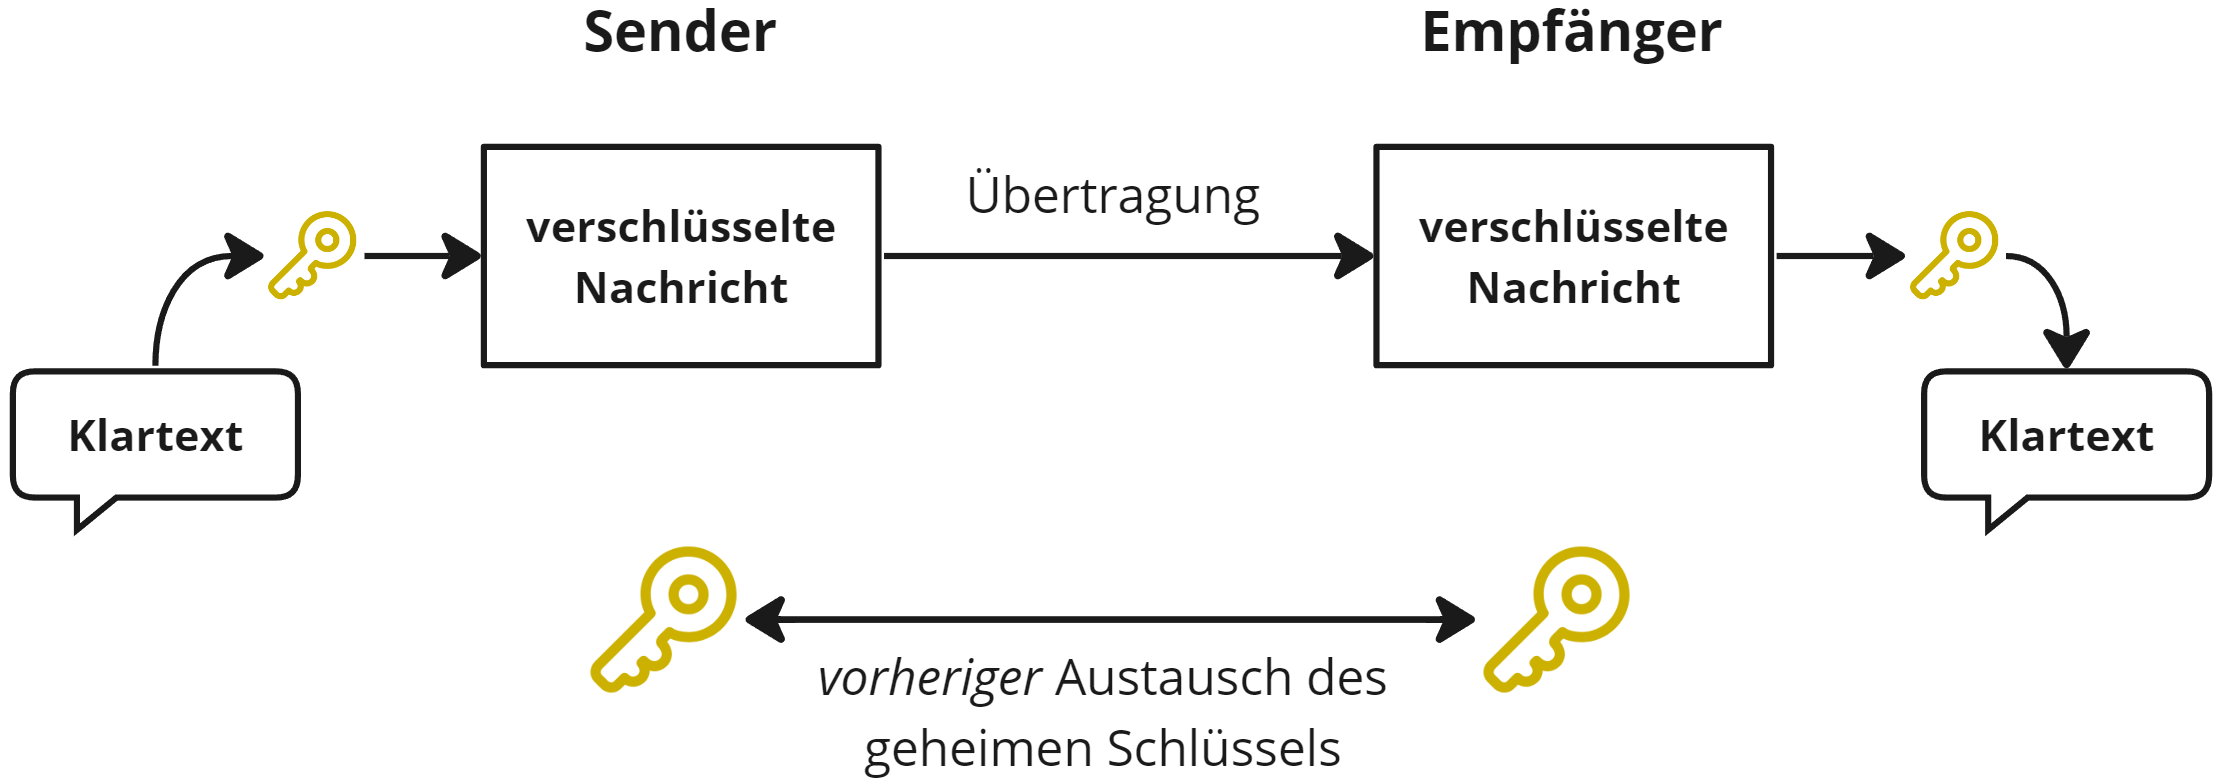
\includegraphics[width=1\linewidth]{images/symmetric_encryption.png}
    \caption{Symmetrische Verschlüsselung (in Anlehnung an \cite{ElektronikKompendium_symmetrischeVerschluesselung})}
    \label{fig:symmetrische_verschluesselung}
\end{center}

\noindent Das Problem bei der symmetrischen Kryptografie ist, dass der Schlüssel zu Beginn der Kommunikation vom Sender an den Empfänger gelangen muss. Dies stellt eine Herausforderung dar, wenn Sender und Empfänger sich noch nicht kennen und noch nie zuvor miteinander kommuniziert haben oder noch nicht über andere Wege einen Schlüssel ausgetauscht haben. Sollte der Schlüssel bei der Übertragung über einen unsicheren Kanal abgefangen werden, kann der Angreifer die Kommunikation entschlüsseln und somit mitlesen \Parencites[S. 644]{DiffieHellman_NewDirectionsInCryptography}[S. 5-8]{Wong_KryptoPraxis}. 

In diesem Fall kann eine Schlüsselvereinbarung verwendet werden, um einen gemeinsamen Schlüssel zu erhalten. Bei der Schlüsselvereinbarung wird ein Schlüssel zwischen zwei Parteien vereinbart, ohne dass dieser über einen unsicheren Kanal übertragen werden muss \Parencite[S. 102]{Wong_KryptoPraxis}. Abbildung \ref{fig:schluesselvereinbarung} zeigt den Ablauf der Schlüsselvereinbarung.

\begin{center}
    \captionsetup{type=figure}
    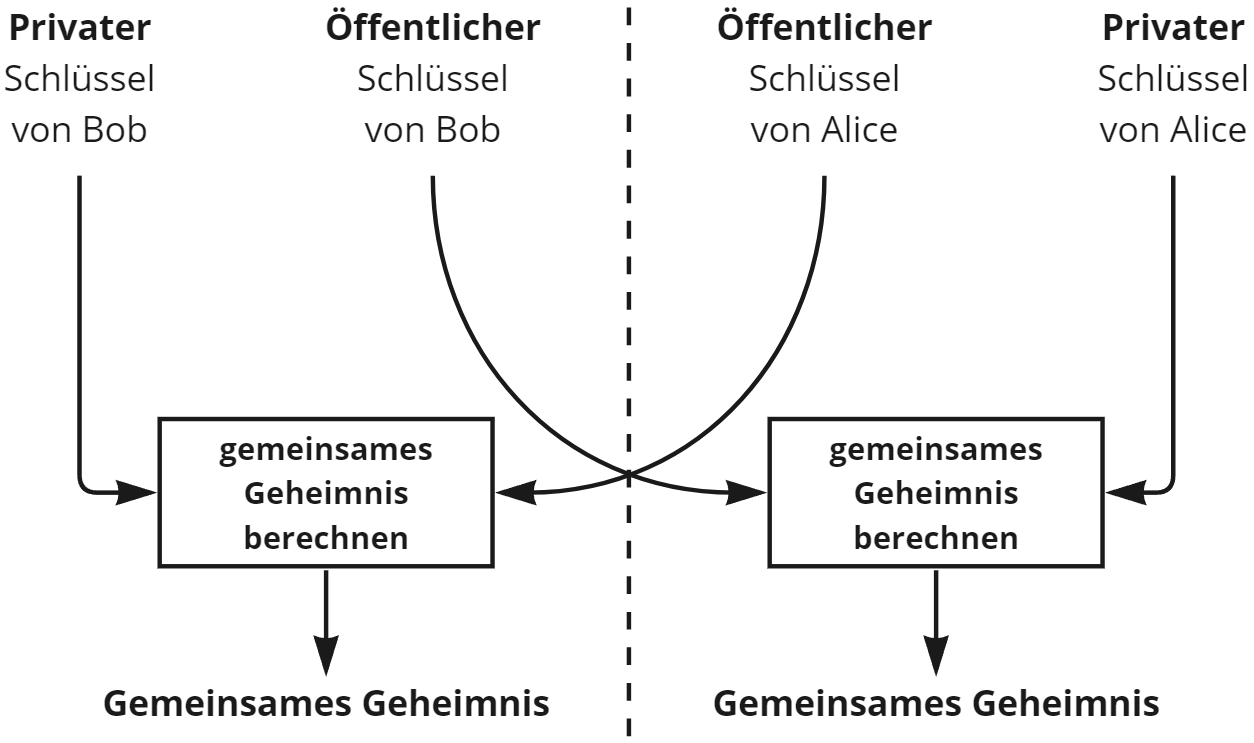
\includegraphics[width=0.7\linewidth]{images/key_exchange.png}
    \caption{Schlüsselvereinbarung (in Anlehnung an \cite[S. 102]{Wong_KryptoPraxis})}
    \label{fig:schluesselvereinbarung}
\end{center}

\noindent Beide Teilnehmer generieren einen privaten Schlüssel und einen öffentlichen Schlüssel. Durch die Kombination des öffentlichen Schlüssels des anderen Teilnehmers und des eigenen privaten Schlüssels wird ein gemeinsames Geheimnis berechnet. Dieses gemeinsame Geheimnis kann dann für die symmetrische Verschlüsselung verwendet werden, da dadurch beide Teilnehmer den gleichen Schlüssel besitzen \Parencite[S. 102]{Wong_KryptoPraxis}.


Bei der \textit{asymmetrische} Kryptografie (auch \textit{Public-Key-Kryptografie} genannt) wird anstatt nur eines Schlüssels ein Schlüsselpaar generiert, das aus einem öffentlichen und einem privaten Schlüssel besteht. Der öffentliche Schlüssel des Empfängers wird zum Verschlüsseln der Nachrichten verwendet und zum Entschlüsseln der Nachrichten wird der private Schlüssel des Empfängers verwendet. Der öffentliche Schlüssel des Empfängers kann von jedem verwendet werden, um Nachrichten an den Empfänger zu verschlüsseln. Nur der Empfänger kann die Nachrichten entschlüsseln, da nur er den privaten Schlüssel besitzt. Der Ablauf der asymmetrischen Verschlüsselung ist in Abbildung \ref{fig:asymmetrische_verschluesselung} dargestellt.


\begin{center}
    \captionsetup{type=figure}
    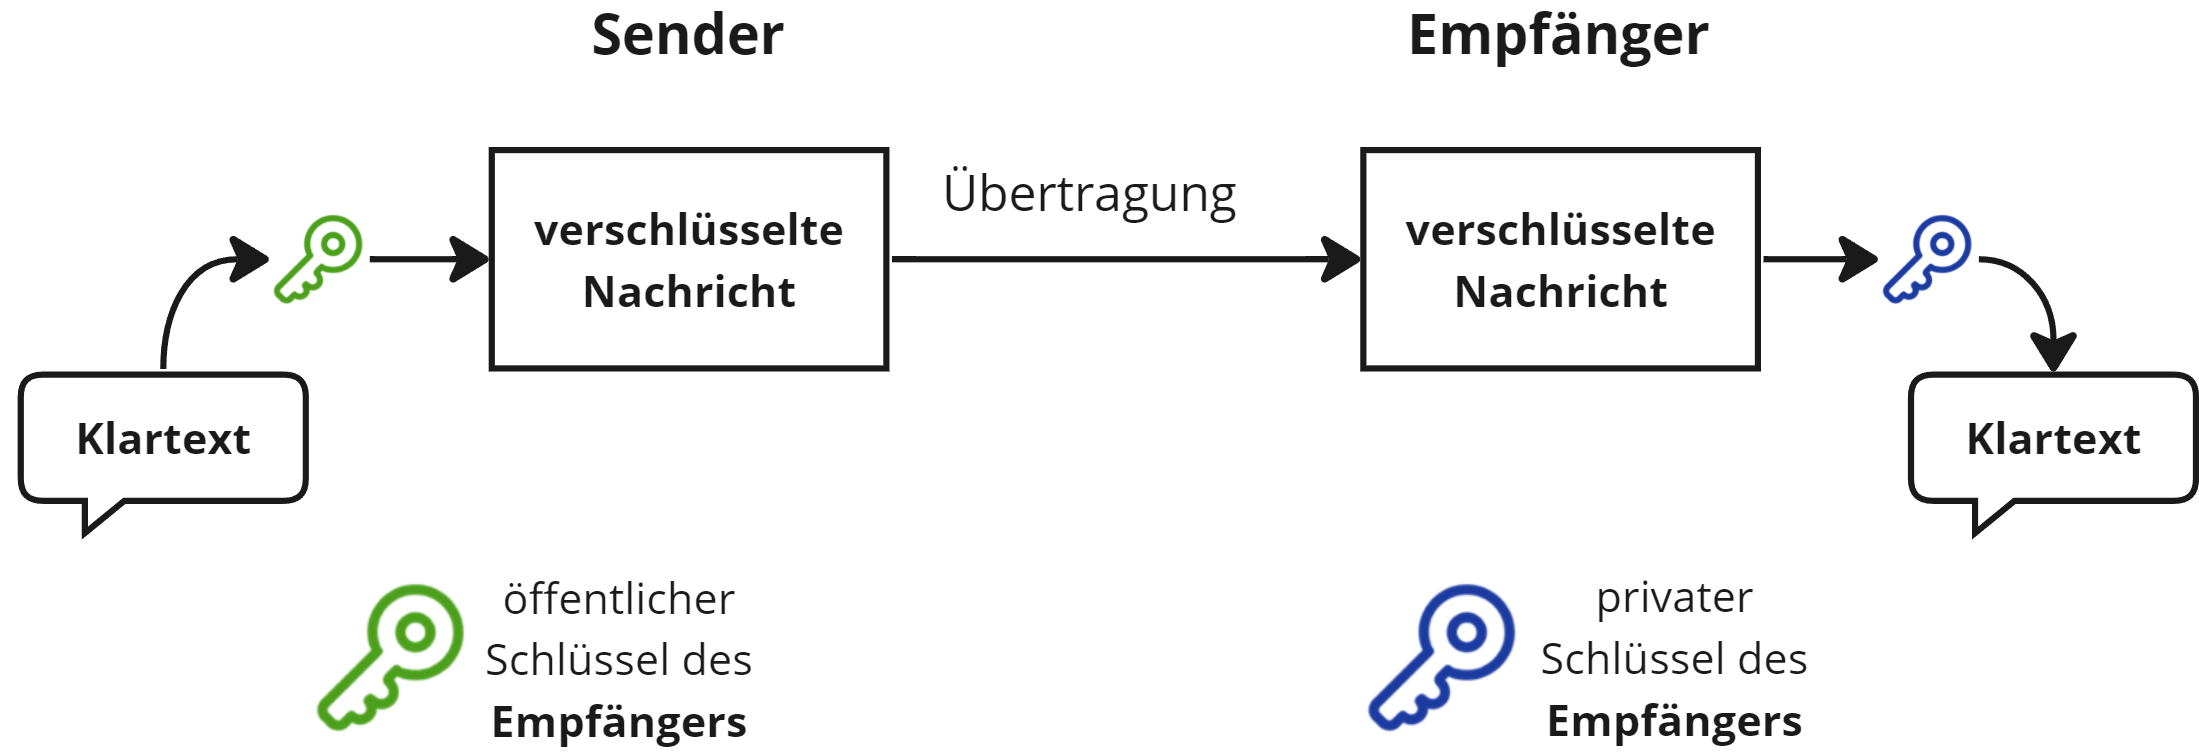
\includegraphics[width=1\linewidth]{images/asymmetric_encryption.png}
    \caption{Asymmetrische Verschlüsselung (in Anlehnung an \cite{ElektronikKompendium_asymmetrischeVerschluesselung})}
    \label{fig:asymmetrische_verschluesselung}
\end{center}

\noindent Es ist außerdem nicht möglich, Nachrichten, die mit dem öffentlichen Schlüssel verschlüsselt wurden, mit diesem auch wieder zu entschlüsseln \parencite{ElektronikKompendium_asymmetrischeVerschluesselung}. 

Diese kryptografische Verfahren können kombiniert werden, um die Vorteile von diesen zu nutzen. Der Schlüsselaustausch wird mit der asymmetrischen Verschlüsselung durchgeführt und die eigentliche Kommunikation wird mit der symmetrischen Verschlüsselung durchgeführt. Dadurch wird die Sicherheit der Kommunikation erhöht, da der Schlüssel nicht über einen unsicheren Kanal übertragen werden muss \Parencite[S. 5-8]{Wong_KryptoPraxis}.


\subsection{Integrität}
\label{subsec:integritaet_signatur}

Um die Integrität der Kommunikation zu gewährleisten, werden digitale Signaturen verwendet. Um den Hash-Wert zu erhalten, wird die Nachricht mit einer Hash-Funktion gehasht. Hash-Funktionen sind Funktionen, die eine Eingabe beliebiger Länge in eine Ausgabe fester Länge umwandeln. Dabei ist es wichtig, dass die Hash-Funktion zwei Eigenschaften erfüllt: \textit{Einwegfunktion} und \textit{Kollisionsresistenz}. Eine Hash-Funktion erfüllt die Eigenschaft der Einwegfunktion, wenn es nicht möglich ist, von der Ausgabe auf die Eingabe zu schließen. Das bedeutet, dass es nicht möglich ist, aus dem Hash-Wert die ursprünglichen Daten zu rekonstruieren. Die Eigenschaft der Kollisionsresistenz ist erfüllt, wenn es nicht möglich ist, zwei verschiedene Eingaben zu finden, die auf den gleichen Hash-Wert abgebildet werden \parencites[S. 12-13]{Brünnler_BlockchainKurzGut}[S. 6]{Fill_BlockchainGrundlagen}. Abbildung \ref{fig:signatur} zeigt, wie eine digitale Signatur funktioniert:

\begin{center}
    \captionsetup{type=figure}
    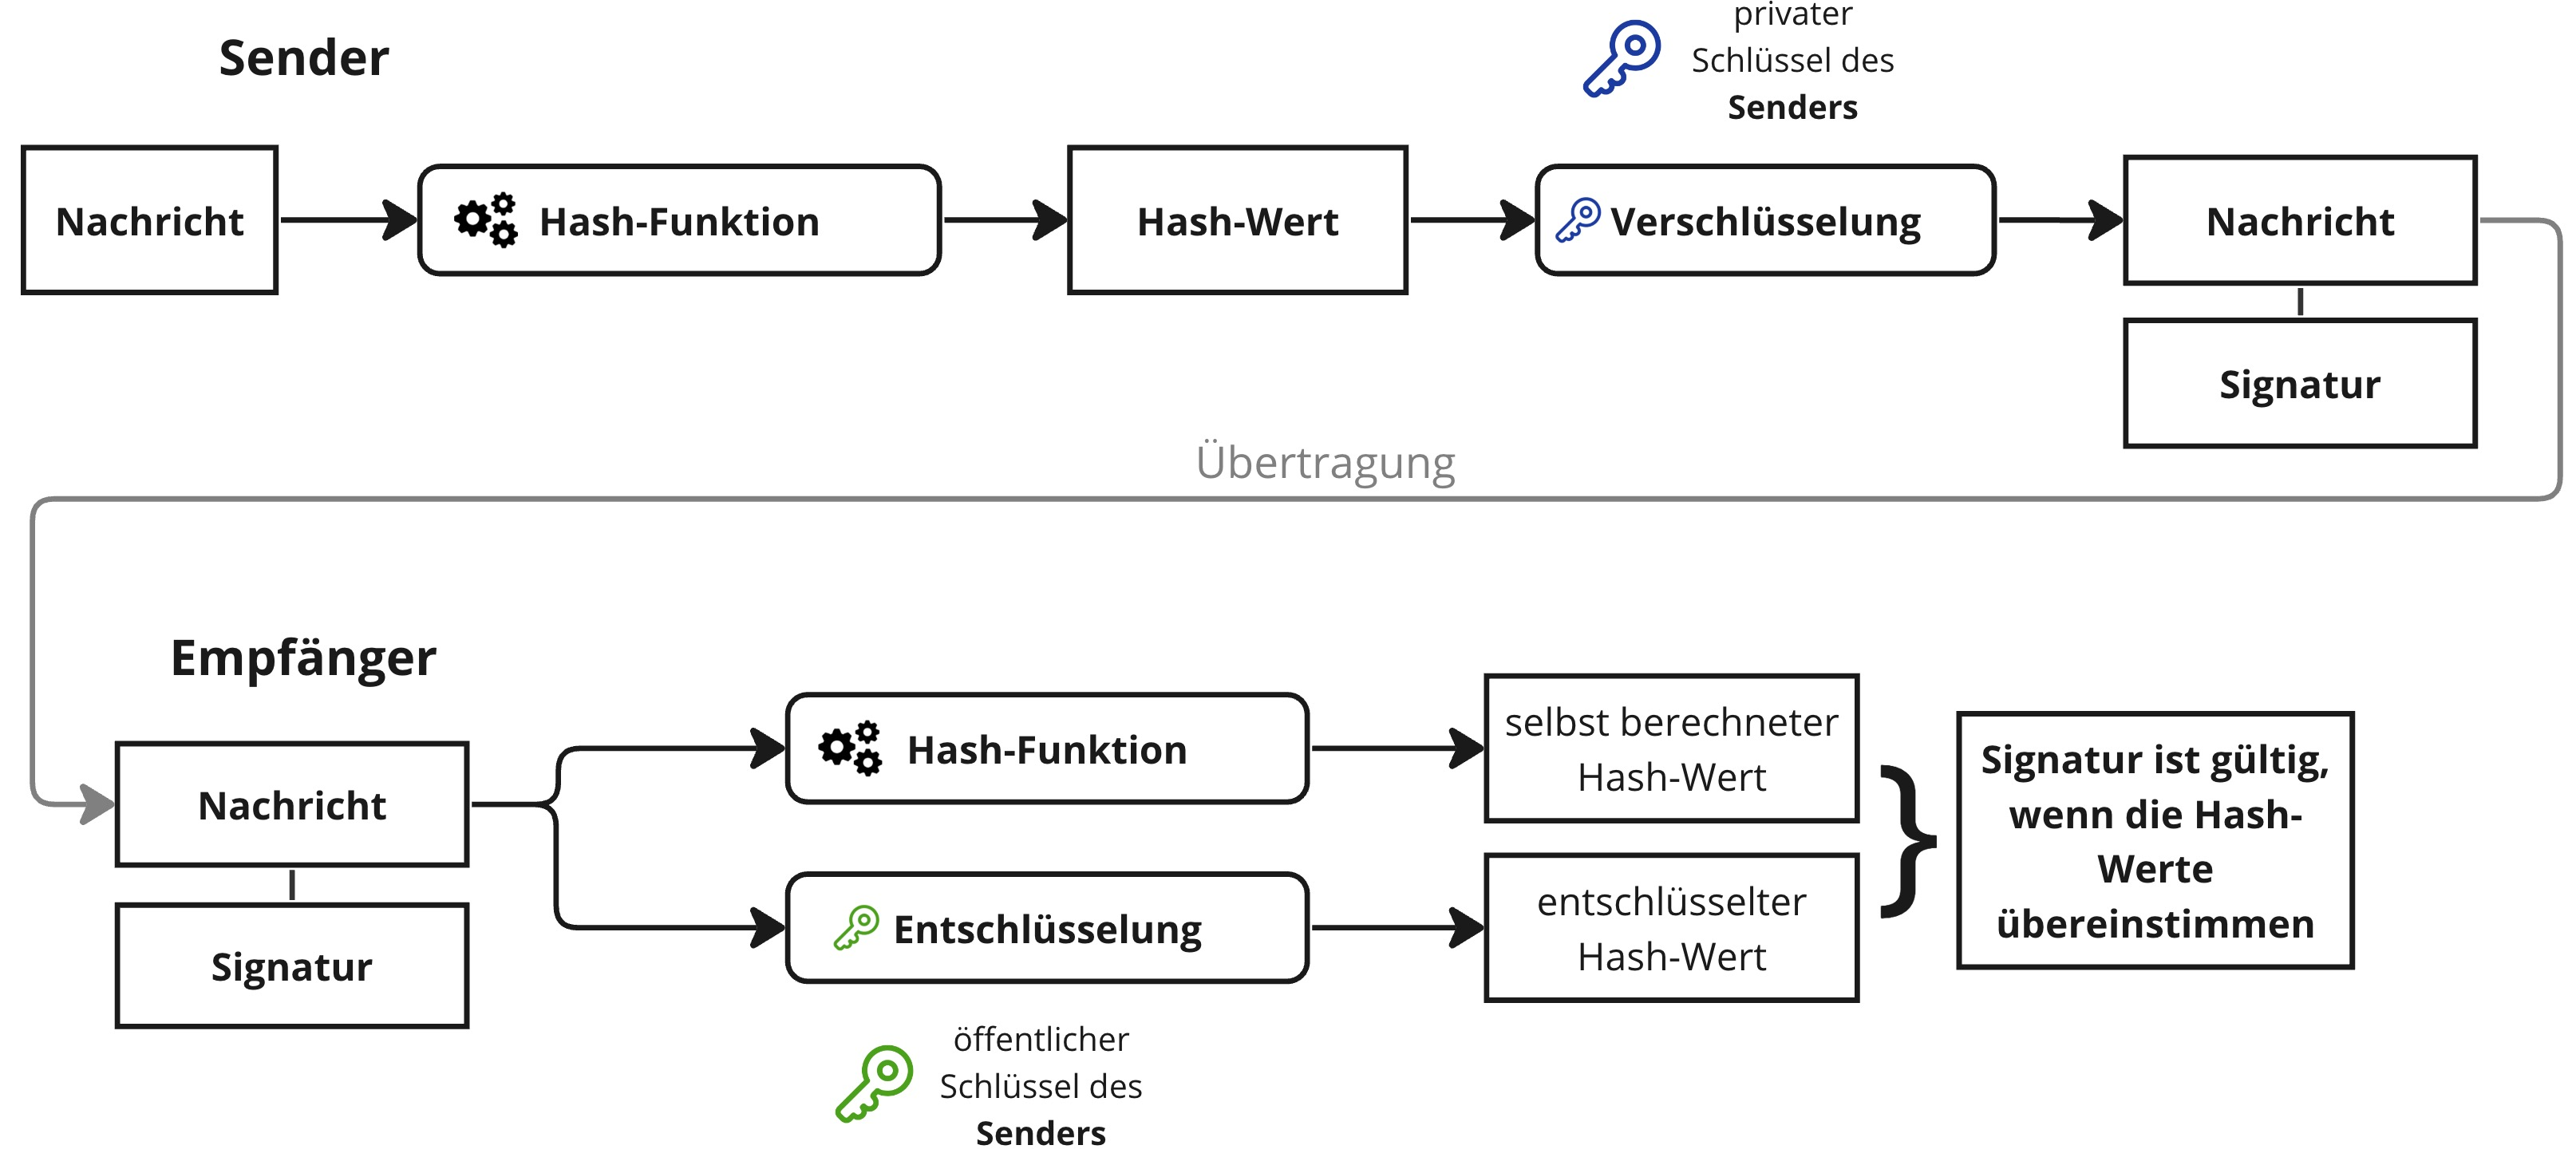
\includegraphics[width=1\linewidth]{images/signatur_2.jpg}
    \caption{Signieren einer Nachricht (in Anlehnung an \cite{DocuSign_digitaleSignaturen})}
    \label{fig:signatur}
\end{center}

% #TODO: Noch erwähnen, dass hier der private schlüssel zum verschlüsseln verwendet wird (anders als bei der asymmetrischen Verschlüsselung)?
\noindent Der Sender berechnet den Hash-Wert der Nachricht, verschlüsselt diesen mit seinem privaten Schlüssel. Das Ergebnis ist die digitale Signatur, welche an die Nachricht angehängt wird. Der Empfänger entschlüsselt den Hash-Wert mit dem öffentlichen Schlüssel des Senders und berechnet den Hash-Wert der Nachricht selbst. Wenn der berechnete Hash-Wert mit dem entschlüsselten Hash-Wert übereinstimmt, kann der Empfänger sicher sein, dass die Nachricht nicht verändert wurde und somit die Integrität der Nachricht gewährleistet ist. Falls der berechnete Hash-Wert nicht mit dem entschlüsselten Hash-Wert übereinstimmt, wurde die Nachricht verändert und die Integrität der Nachricht ist nicht mehr gewährleistet \Parencite[S. 73-78]{Hellmann_IT-Sicherheit}.


\subsection{Authentizität}

Für die Authentizität der Kommunikation werden ebenfalls Signaturen verwendet. Der Sender signiert die Nachricht mit seinem privaten Schlüssel und sendet die signierte Nachricht an den Empfänger. Durch die Integration der Blockchain in dieser Arbeit fungiert diese als öffentliches Verzeichnis oder auch Key-Server, in dem die öffentlichen Schlüssel der Teilnehmer gespeichert sind. Der Empfänger kann den öffentlichen Schlüssel des Senders aus der Blockchain auslesen, wodurch nachvollzogen werden kann, ob die Nachricht vom Sender stammt oder nicht.


\subsection{Ende-zu-Ende-Verschlüsselung am Beispiel des Signal-Protokolls}
\label{subsec:signal_protokoll_basics}

Das Signal-Protokoll nutzt verschiedene fortschrittliche Verschlüsselungstechniken, um eine durchgängige Ende-zu-Ende-Verschlüsselung sicherzustellen. Für den Austausch von Schlüsseln bedient sich Signal des sogenannten \textit{Double Ratchet Algorithmus}. Dieser Algorithmus ist eine kryptografische Methode, um Ende-zu-Ende-Verschlüsselung und \textit{Perfekte Zukunftssicherheit}, auch \textit{Perfect Forward Secrecy} genannt, zu ermöglichen. Es werden zwei Arten von Schlüsselpaaren verwendet: ein \textit{statisches} Schlüsselpaar, das für Authentifizierungszwecke dient, und ein \textit{flüchtiges} beziehungsweise \textit{ephemeres} Schlüsselpaar, das für die eigentliche Verschlüsselung der Nachrichten genutzt wird. Der Double Ratchet Algorithmus integriert zudem einen \textit{Root Key}, der für die Verschlüsselung der übermittelten Nachrichten verantwortlich ist und dessen Vereinbarung mittels Diffie-Hellman-Schlüsselaustausch erfolgt. Der Root Key wird nur einmal vereinbart und wird für die gesamte Kommunikation verwendet. Die Abbildung \ref{fig:double_ratchet} zeigt einen vereinfachten Ablauf des Double Ratchet Algorithmus.


\begin{center}
    \captionsetup{type=figure}
    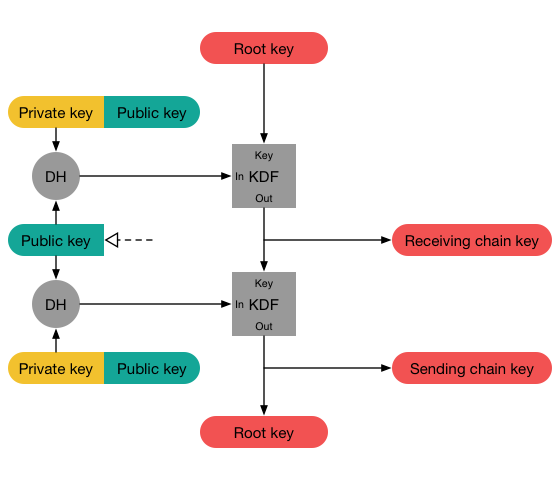
\includegraphics[width=0.8\linewidth]{images/double_ratchet.png}
    \caption{Double Ratchet Algorithmus \parencite{Signal_DoubleRatchet}}
    \label{fig:double_ratchet}
\end{center}


\noindent Nach der Vereinbarung des Root Keys wird dieser genutzt, um einen \textit{Chain Key} zu generieren. Der Chain Key wiederum wird dazu verwendet, einen \textit{Message Key} zu erzeugen, welcher die eigentliche Verschlüsselung der Nachrichten ermöglicht. Das Kernelement dieses Algorithmus ist das \textit{Key Ratcheting}. Der Begriff \textit{Ratchet} (zu Deutsch: \textit{Ratsche}) bezeichnet ein Werkzeug, das nur in eine Richtung gedreht werden kann. Das Key Ratcheting bezeichnet also die Eigenschaft, dass die Schlüssel nur in eine Richtung geändert werden können und es somit unmöglich ist, vorherigen Schlüssel zu berechnen. Der Chain Key wird nach dem Empfang jeder Nachricht aktualisiert, indem er mittels erneutem Diffie-Hellman-Schlüsselaustausch und dem Root Key neu berechnet wird. Gleichzeitig wird der Message Key nach jeder übermittelten Nachricht aktualisiert, indem er durch erneuten Diffie-Hellman-Schlüsselaustausch und unter Einbeziehung des Chain Keys neu generiert wird. Dadurch wird sichergestellt, dass jeder Message Key nur einmal verwendet wird und somit die \textit{Perfect Forward Secrecy} gewährleistet ist \parencite{Signal_DoubleRatchet}. 

Die Perfect Forward Secrecy definiert die Eigenschaft, dass die Parameter während der Kommunikation ständig neu berechnet werden und somit die Sicherheit der Kommunikation auch dann gewährleistet ist, wenn ein Angreifer in der Zukunft den privaten Schlüssel eines Teilnehmers erlangt \parencite{ElektronikKompendium_PFS}.
